\documentclass[10pt]{beamer}
\usepackage{pgf}
\usepackage{booktabs}
%Information to be included in the title page:
\title{Elite individuals, insitutions, and economic growth accounting}
\author{James Xu}
\institute{ECON 442, Duke University}
\date{2024}
\usefonttheme[onlymath]{serif}

\begin{document}
\setbeamertemplate{navigation symbols}{}

\frame{\titlepage}

\begin{frame}
    \frametitle{Research Question}
    \begin{block}{What is the relationship between elite students, academic institutions, and economic growth?}
        \begin{itemize}
            \item Are there outsized returns to economic growth when there are more academic elites?
            \item How can we measure academic competition and education quality beyond means?
        \end{itemize}
    \end{block}
    \begin{exampleblock}{Method}
        Through this paper, I investigate the relationship between the number of top-ranked universities, share of top math students,
        IMO scores, and GDP per capita growth to analyze these questions.
    \end{exampleblock}
\end{frame}

\begin{frame}
\frametitle{Data Sources}
\begin{itemize}
    \item World Bank: World Development Indicators
    \item International Math Olympiad
    \item ARWU University Rankings
    \item PISA Math Scores
    \item Economist Democracy Scores
\end{itemize}
\end{frame}

\begin{frame}{World Bank Data}
    The World Bank collects and publishes development indicators for most countries/economies in the world. In this paper, I use the following variables:

    \begin{itemize}
        \item GDP Per Capita Growth: \% growth in constant 2015 \$USD
        \item GDP Per Capita: current \$USD
        \item School Completion Rates: \% gross of relevant age group
        \begin{itemize}
            \item ``What \% of primary-school-aged population is enrolled in primary school?''
            \item This number can be greater than 100\%
            \item Not available for all years and all countries $\rightarrow$ missing data problem
        \end{itemize}
        \item Population: all residents of a country/territory
    \end{itemize}
\end{frame}

\begin{frame}
    \frametitle{World Bank Data}
    \framesubtitle{Distributions}
    \centering
    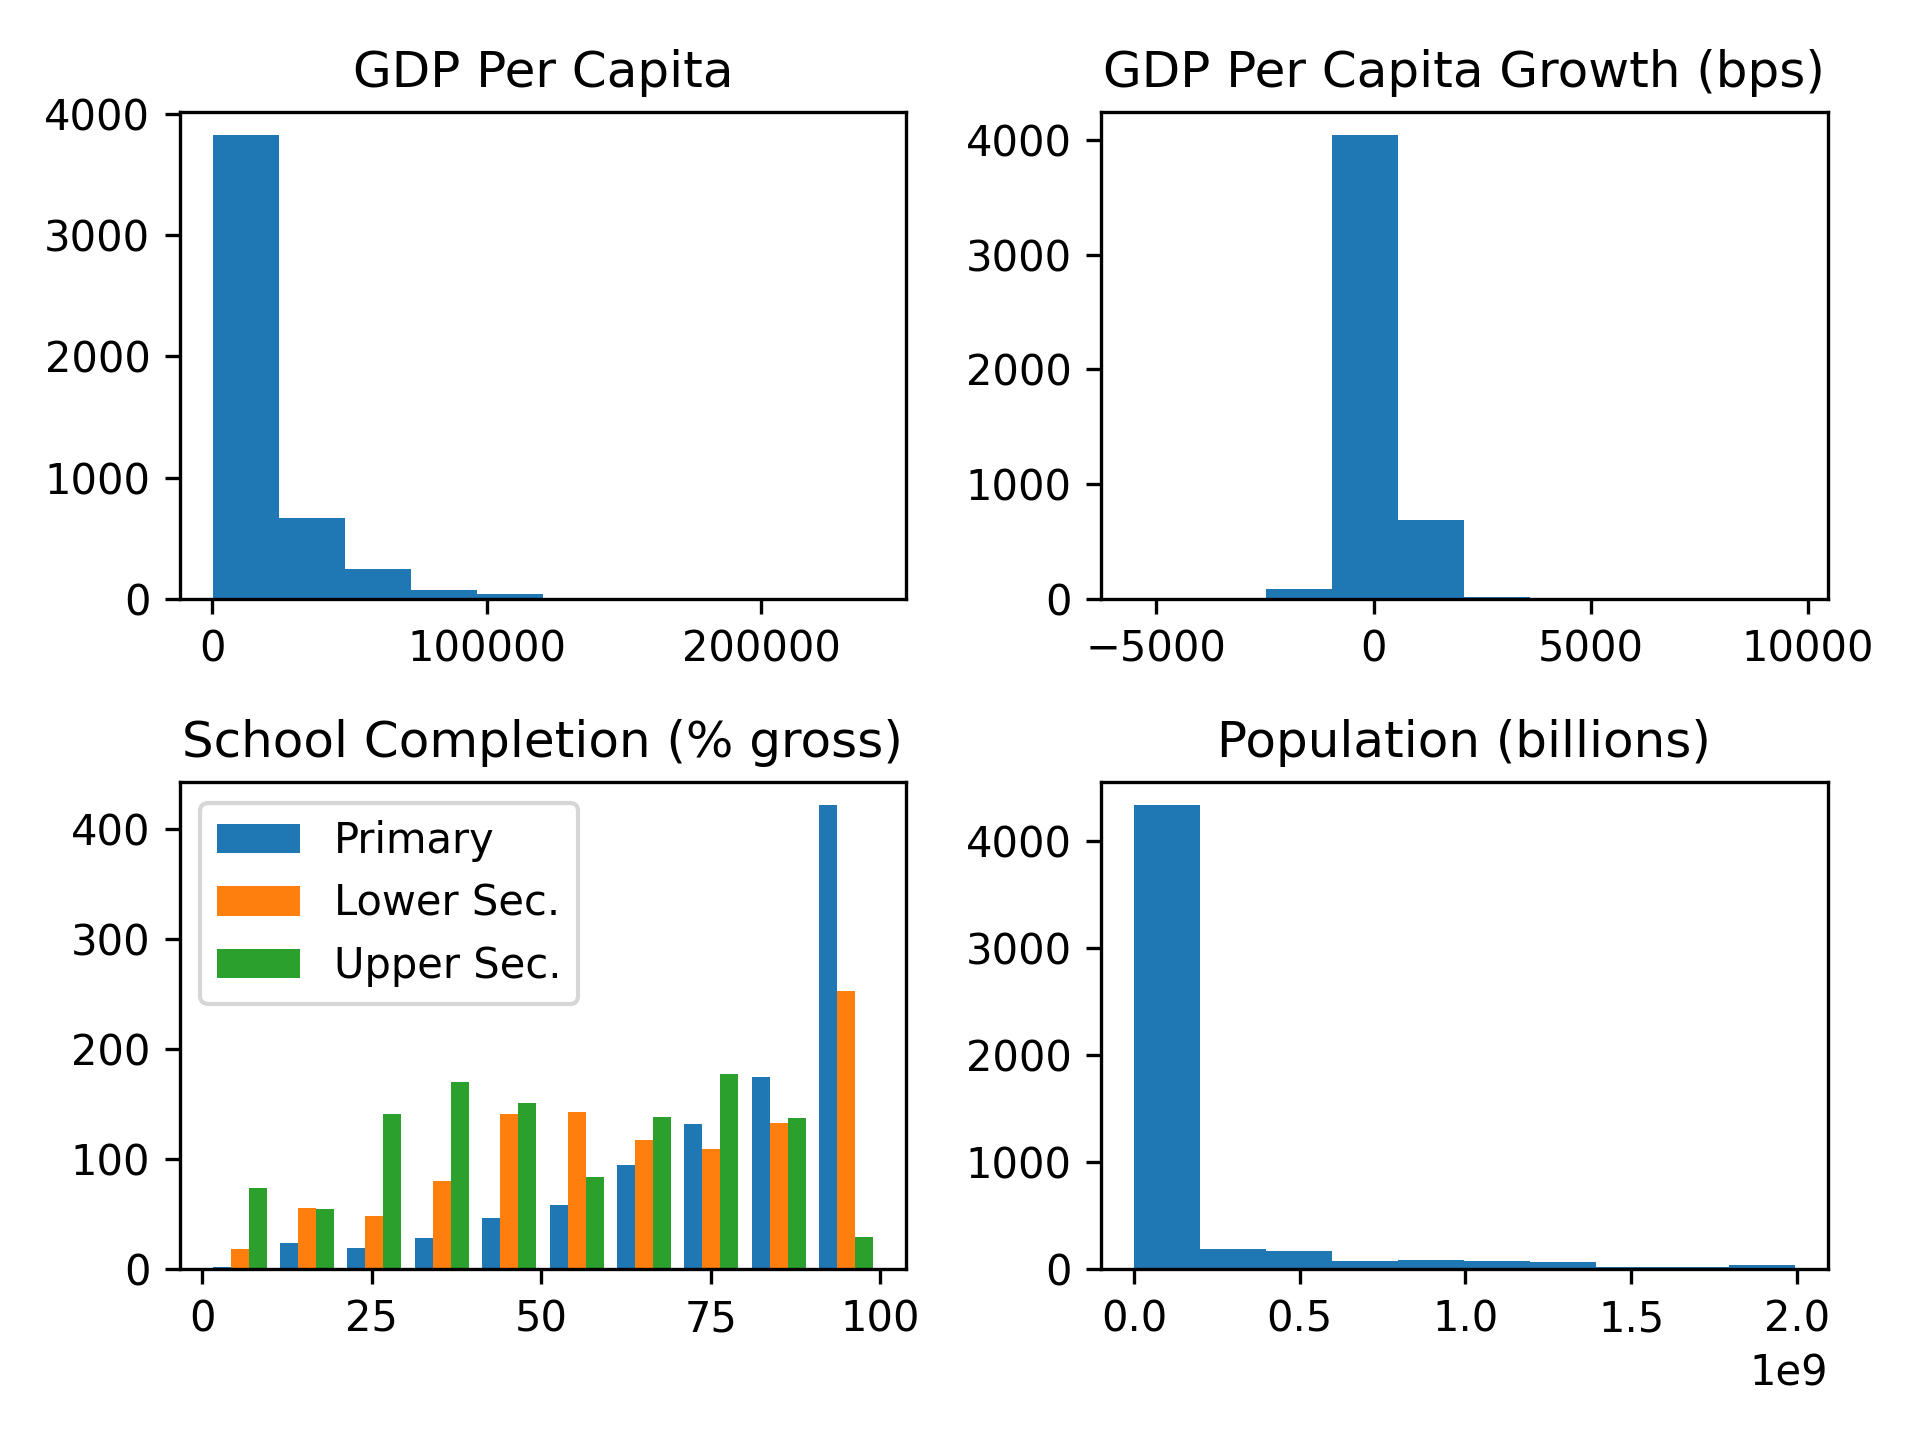
\includegraphics[width=\textwidth]{../charts/wdi.png}
\end{frame}

\begin{frame}
    \frametitle{World Bank Data}
    \framesubtitle{Missing data}
    \centering
    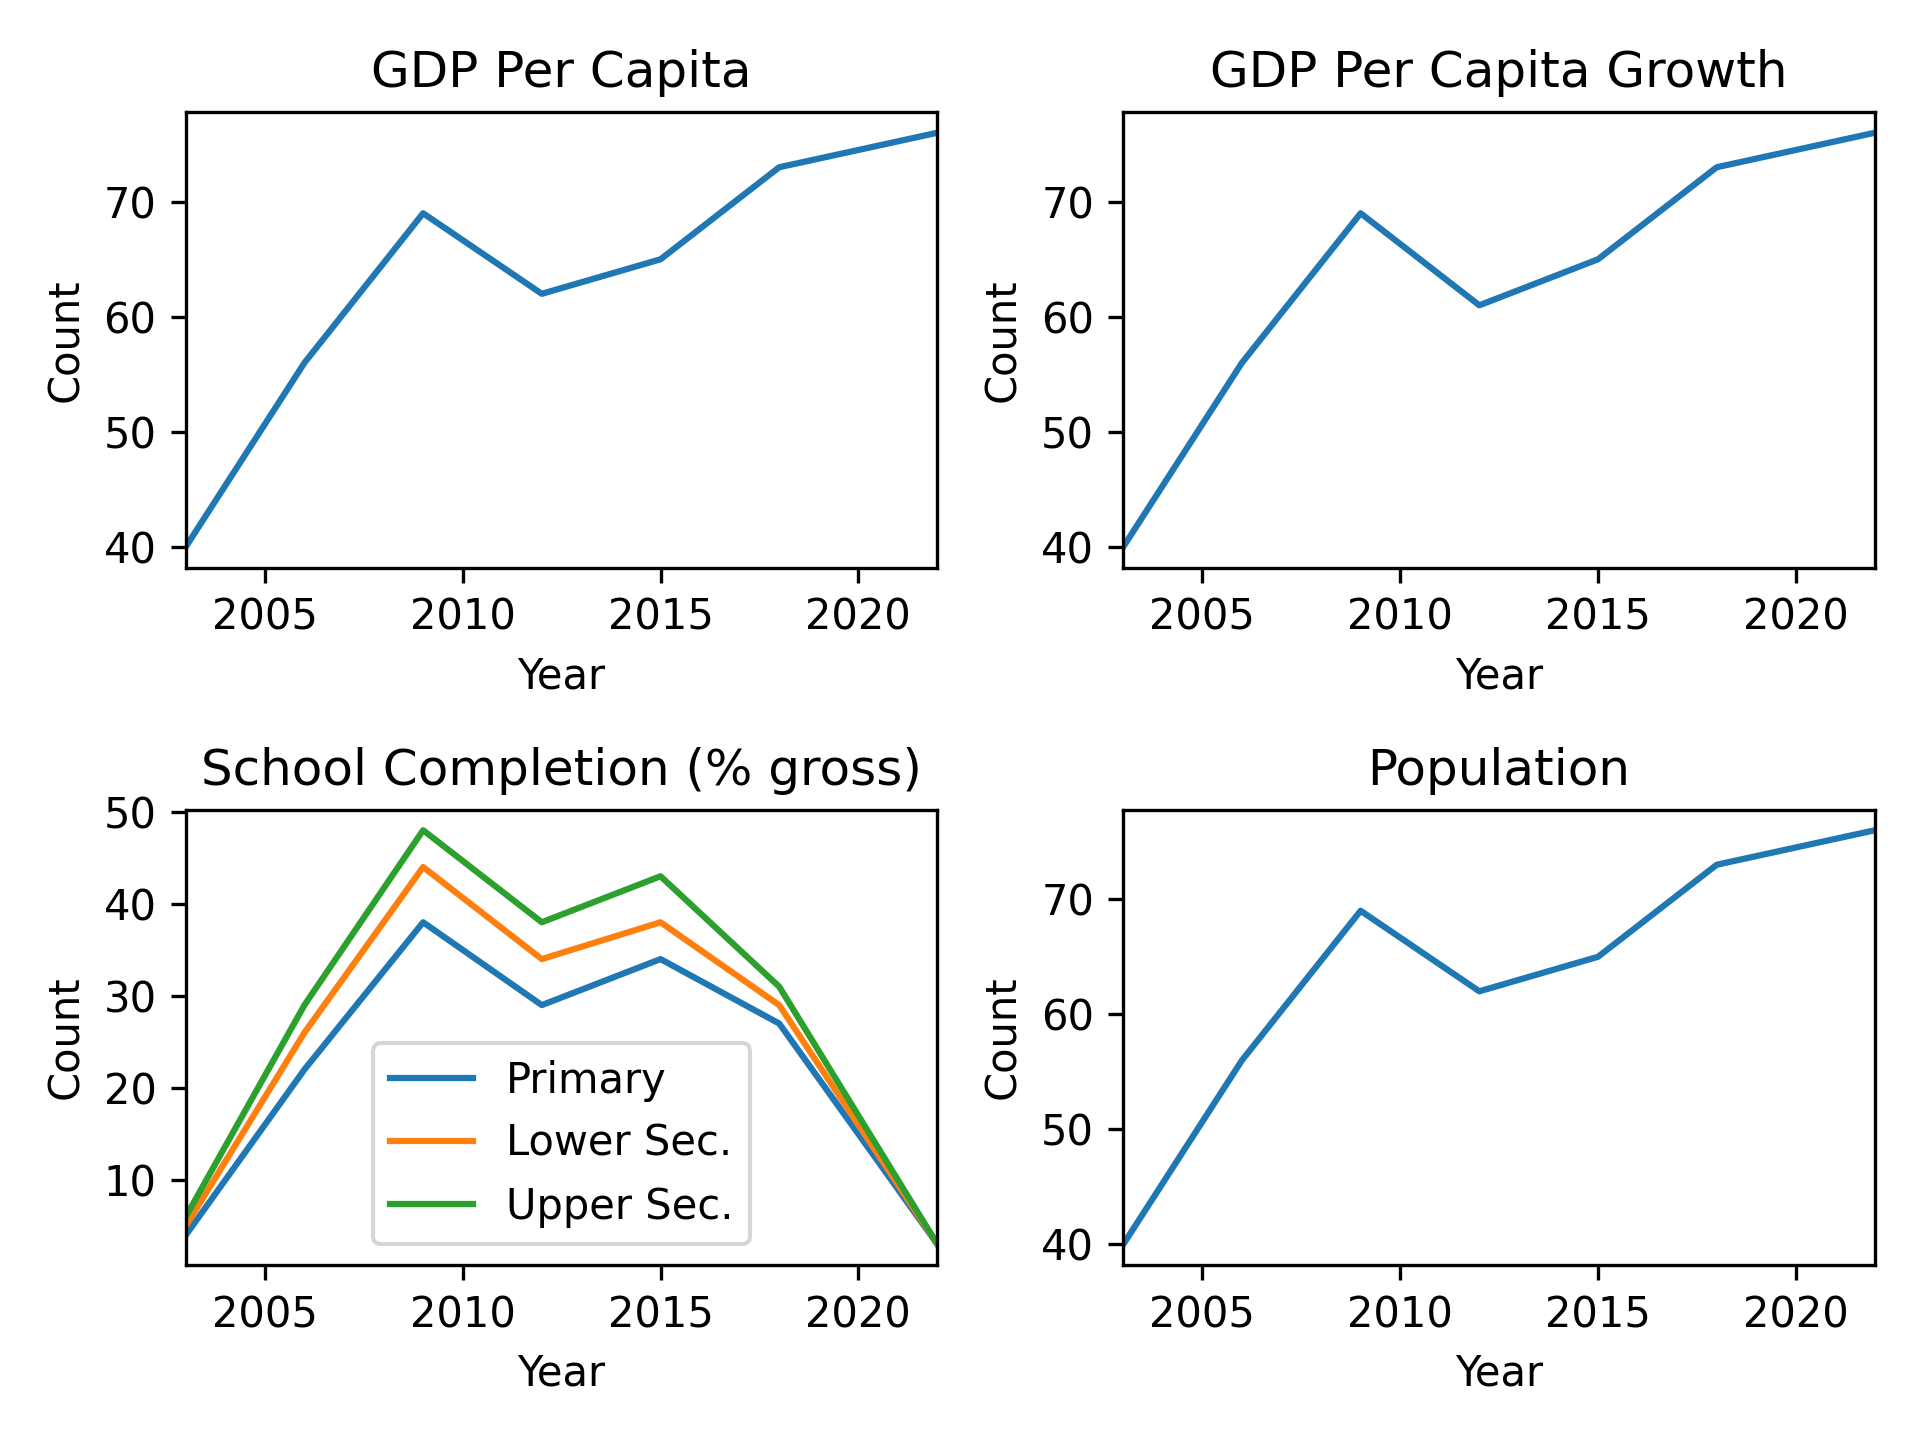
\includegraphics[width=\textwidth]{../charts/wdi-count.png}
\end{frame}

\begin{frame}{Imputing nulls}{Using XGBoost for better predictions}
    \begin{block}{Data is not missing at random}
        School completion data is only available for a maximum of 80 countries per year and has high variance in this availablility.
        This is the most limiting factor in the analysis.
    \end{block}

    \begin{block}{Predicting missing values}
        XGBoost is a tree-based model that has built-in null handling. I use the remaining variables to predict school completion rates.
        Achieves significantly higher accuracy than linear regression.
    \end{block}
    
\end{frame}

\begin{frame}{Imputation results}
    \centering
    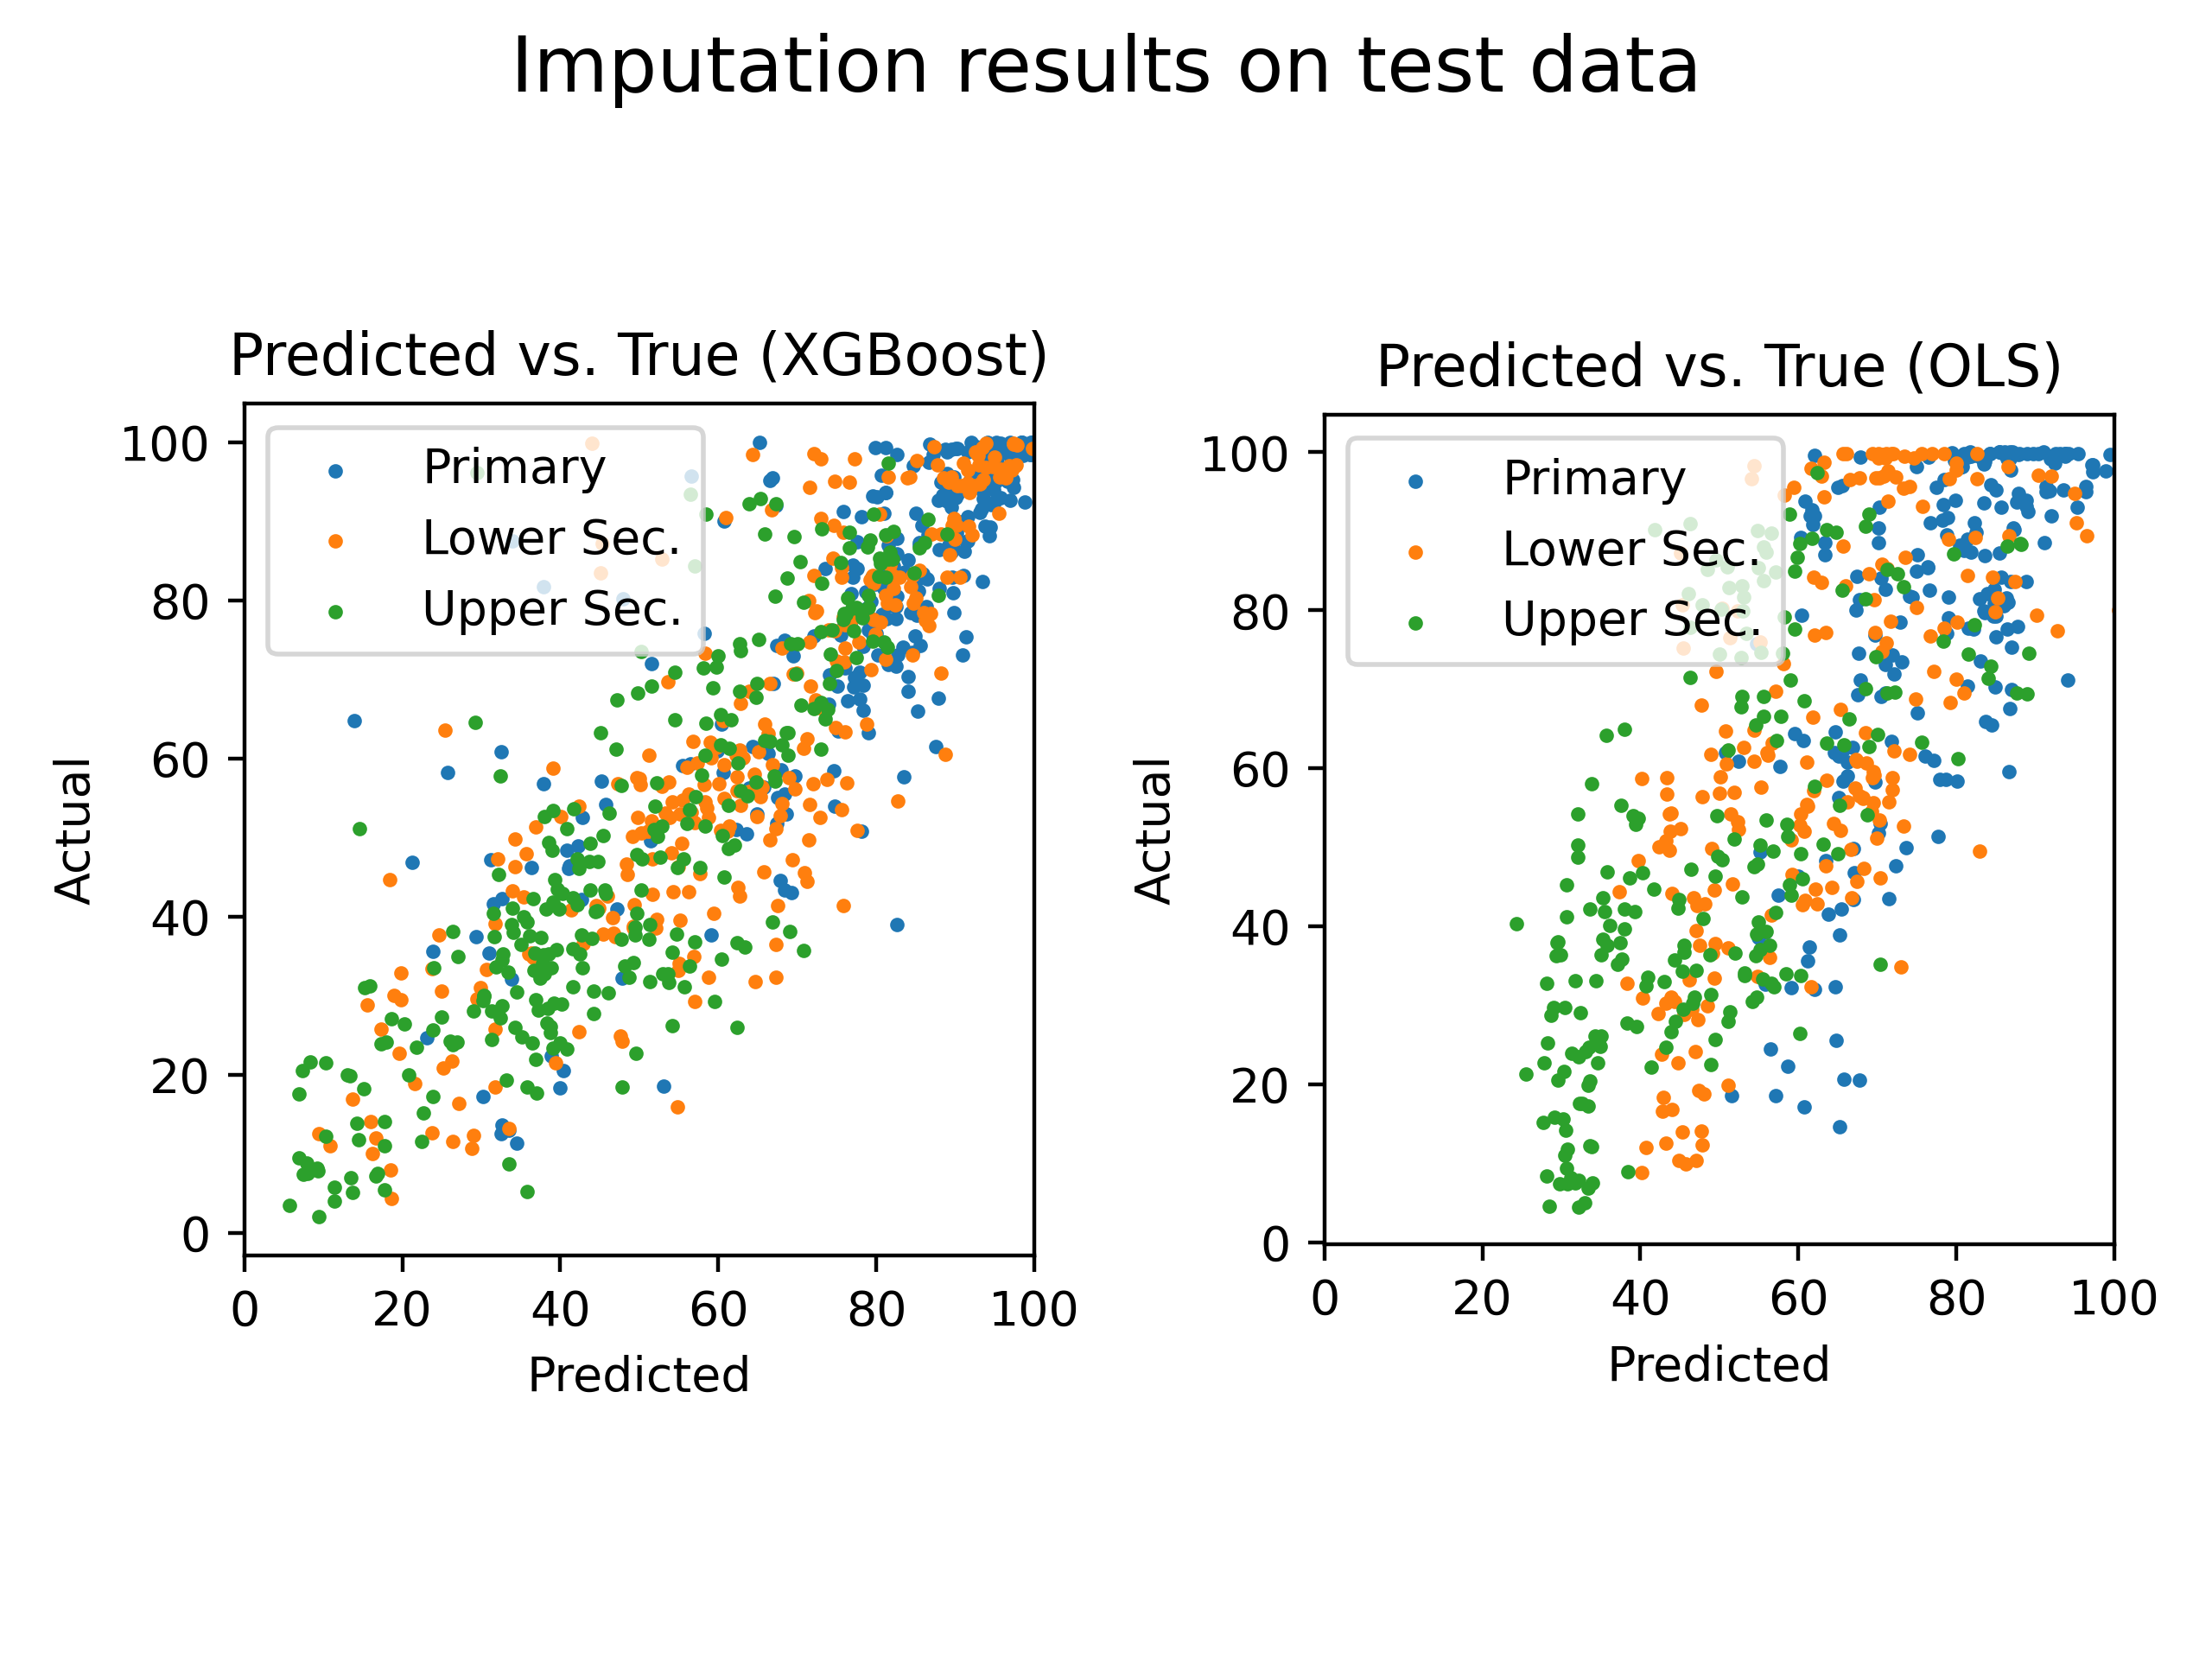
\includegraphics[width=\textwidth]{../build/xgboost.png}
\end{frame}

\begin{frame}{IMO Scores}{The IMO is an international mathematics contest for high school students
    }
    \begin{columns}
        \column{0.5\textwidth}
            \centering
            \begin{table}
            \caption{Top 10 countries by IMO score.}
            \resizebox{\textwidth}{!}{
            \begin{tabular}{lrrr}
                \toprule
                 & IMO Score & GDPpc & GDPpc Growth \\
                Region &  &  &  \\
                \midrule
                KOR & 10.2026 & 26060.9203 & 293.8552 \\
                CHN & 9.8296 & 6424.4972 & 786.8171 \\
                USA & 9.6196 & 54346.5078 & 125.7613 \\
                RUS & 9.0800 & 10432.8366 & 277.0704 \\
                SGP & 9.0642 & 51652.4651 & 348.0543 \\
                BGR & 8.8821 & 7556.3933 & 417.7564 \\
                ROU & 8.7367 & 9432.6698 & 439.7522 \\
                HUN & 8.7153 & 13979.7009 & 262.9650 \\
                VNM & 8.5029 & 2159.2583 & 527.6404 \\
                UKR & 8.3941 & 3079.8378 & 131.9303 \\
                \bottomrule
            \end{tabular}}
        \end{table}
        \column{0.5\textwidth}
            \begin{itemize}
                \item Scores collected from 2003 to 2022
                \item Scores are transformed by $t(s) = \frac{s}{\log P}$ where $s$ is the country's raw score and $P$ is population.
                \begin{itemize}
                    \item Team size of 6 means that larger countries have an advantage due to ``genius odds''
                    \item Score is capped, so dividing by $\log P$ will correct for theoretical ceiling of performance
                \end{itemize}
            \end{itemize}
        \end{columns}
\end{frame}

\begin{frame}{ARWU Rankings}{Description and Usage}
    ARWU (Academic Ranking of World Universities) is a set of university rankings based primarily on research output.
    \begin{itemize}
        \item Rankings are produced annually and are available from 2003
        \item From 2003 to 2016, 500 top universities were ranked; after 2017, 1000 were ranked.
    \end{itemize}
    
    \begin{block}{Per-Capita Scaling}
        Larger countries naturally have an advantage, so a more fair metric is
        \[ARWU_{i,t} = \frac{arwuCount_{i,t}}{P_{i,t}} \cdot 10^6 \]
        Instead, looking at ARWU insitutions per million population indicates the relative quantity of elite insitutions in a country/region.
    \end{block}
    
\end{frame}

\begin{frame}{Summary Statistics}
    Hello
\end{frame}

\begin{frame}{Rationale for variables}
    \begin{block}{IMO Scores}
        Indicator for a country's (and region's) ability to develop/identify pinncale STEM talent at high school level.
    \end{block}

    \begin{block}{ARWU Rankings}
        Indicator for a country's (and region's) ability to produce exellence in research output.
    \end{block}

    \begin{block}{Percent in PISA 99th percentile}
        When controlling for average PISA math scores, this is a partial indicator for whether general excellence in academics is encouraged/necessary.
    \end{block}
\end{frame}

\begin{frame}{Model specification}
    Let variables of interest be: $math99, ARWU, ARWU \times GDPpc, IMO$.
    For the sake of concision, let $E$ be a 1 by 4 matrix defined as:
    \[E_{i,t} = 
    \begin{bmatrix}
        math99_{i, t} & ARWU_{i, t} & ARWU_{i, t} \times GDPpc_{i, t} & IMO_{i, t}
    \end{bmatrix}
    \]
    Let the coefficients of $E_{i, t}$ be a 4 by 1 matrix called $\lambda$. For control variables, $C_{i, t}$ is the matrix of variables and $\alpha$ is coefficients..
    \begin{equation}
        Y_{i, t} = \beta_0 + \lambda E_{i, t} + \alpha C_{i, t} + T_t + \epsilon_{i, t}
    \end{equation}
    Due to missing data, consider another regression model which does not include $math99, math$:
    \begin{equation}
        Y_{i, t} = \alpha_0 + \lambda_{np} Enp_{i, t} + \alpha_{np} Cnp_{i, t} + T_t + \epsilon_{i, t}
    \end{equation}
    where $Y_{i,t}$ is GDP per capita growth in basis points. Time effects are included to control for secular changes (e.g. business cycles).
\end{frame}

\begin{frame}{Relationships}
    Insert scatter plots for each of 3 key variables.
\end{frame}

\begin{frame}{PISA data regression}{Highly dependent on model specification due to rich country bias and limited variation}
    \begin{table}[!htbp] \centering
        \resizebox{\linewidth}{!} {
            \begin{tabular}{@{\extracolsep{2pt}}lcccc}
                \\[-1.8ex]\hline
                \hline \\[-1.8ex]
                & \multicolumn{4}{c}{\textit{Dependent variable: GDPpcGrowth}} \
                \cr \cline{2-5}
                \\[-1.8ex] & (1) & (2) & (3) & (4) \\
                \hline \\[-1.8ex]
                 PISA Math in global P99 & & 12.582$^{}$ & 16.888$^{}$ & 122.288$^{}$ \\
                & & (23.160) & (20.869) & (79.814) \\
                 IMO score per log population & 11.744$^{}$ & 4.247$^{}$ & 10.055$^{}$ & 71.462$^{**}$ \\
                & (7.232) & (9.102) & (8.154) & (29.447) \\
                 ARWU insitutions & -586.307$^{***}$ & -559.067$^{**}$ & -575.550$^{***}$ & -295.306$^{}$ \\
                & (198.985) & (240.047) & (213.365) & (559.483) \\
                 ARWU insitutions x GDP PC & 0.009$^{**}$ & 0.009$^{*}$ & 0.008$^{*}$ & -0.007$^{}$ \\
                & (0.004) & (0.005) & (0.004) & (0.014) \\
                 PISA Math & & 0.636$^{}$ & -0.273$^{}$ & -4.581$^{}$ \\
                & & (0.949) & (0.876) & (3.456) \\
                 GDP per capita & -0.003$^{**}$ & -0.006$^{***}$ & -0.004$^{**}$ & -0.007$^{}$ \\
                & (0.002) & (0.002) & (0.002) & (0.012) \\
                 Primary School Completion Rate & -0.712$^{}$ & -2.406$^{}$ & -0.112$^{}$ & -4.624$^{}$ \\
                & (3.868) & (4.849) & (4.338) & (18.411) \\
                 Lower Sec. Completion Rate & 1.485$^{}$ & 0.777$^{}$ & 1.568$^{}$ & 21.092$^{}$ \\
                & (3.255) & (3.704) & (3.290) & (16.364) \\
                 Upper Sec. Completion Rate & 1.597$^{}$ & 1.439$^{}$ & 1.542$^{}$ & -15.224$^{}$ \\
                & (2.515) & (2.870) & (2.543) & (17.185) \\
                 Democracy Rating & 0.940$^{}$ & 3.972$^{}$ & 4.167$^{}$ & -12.702$^{}$ \\
                & (19.787) & (23.684) & (21.249) & (128.289) \\
                 Time Effects & Yes & No & Yes & Yes \\
                 Fixed Effects & No & No & No & Yes \\
                 Entities & 48 & 48 & 48 & 48 \\
                \hline \\[-1.8ex]
                 Observations & 109 & 109 & 109 & 109 \\
                 $R^2$ & 0.397 & 0.212 & 0.402 & 0.753 \\
                 Adjusted $R^2$ & 0.322 & 0.122 & 0.313 & 0.432 \\
                 Residual Std. Error & 197.737 (df=96) & 224.993 (df=97) & 199.076 (df=94) & 181.047 (df=47) \\
                 F Statistic & 5.275$^{***}$ (df=12; 96) & 2.367$^{**}$ (df=11; 97) & 4.512$^{***}$ (df=14; 94) & 2.345$^{***}$ (df=61; 47) \\
                \hline
                \hline \\[-1.8ex]
                \textit{Note:} & \multicolumn{4}{r}{$^{*}$p$<$0.1; $^{**}$p$<$0.05; $^{***}$p$<$0.01} \\
                \end{tabular}
        }
        \end{table}
\end{frame}

\begin{frame}{Interpreting Regressions}{PISA regressions}
    Regression results do not present a clear picture of the existence of a statistical relationship between elite indicators and economic growth.
    \begin{block}{Little variation in data}
        \begin{itemize}
            \item Countries and regions with PISA test scores tend to be wealthier, more developed economies
            \item Low variance within countries over time and between countries as a result
        \end{itemize}
    \end{block}

    \begin{block}{Model specification matters}
        \begin{itemize}
            \item Including entity fixed effects makes the most significant difference versus time effects (likely due to above)
            \item Magnitudes of $math99$ is 10x larger when entity fixed effects are included; similar for $IMO$
            \item $ARWU$ and interaction terms reversed in sign compared to not including fixed effects
            \begin{itemize}
                \item Possibly due to omitted variable bias that is captured by fixed effects
            \end{itemize}
        \end{itemize}

    \end{block}
    
\end{frame}

\begin{frame}
    \frametitle{Non-PISA data regression}
    \begin{table}[!htbp] \centering
        \resizebox{\linewidth}{!} {
            \begin{tabular}{@{\extracolsep{5pt}}lcccc}
                \\[-1.8ex]\hline
                \hline \\[-1.8ex]
                & \multicolumn{4}{c}{\textit{Dependent variable: GDPpcGrowth}} \
                \cr \cline{2-5}
                \\[-1.8ex] & \multicolumn{1}{c}{Model 3 (PISA)} & \multicolumn{1}{c}{Model 5 (PISA years)} & \multicolumn{1}{c}{Model 6 (All years)} & \multicolumn{1}{c}{Model 7 (All years, FE)}  \\
                \hline \\[-1.8ex]
                 IMO score per log population & 10.055$^{}$ & 18.160$^{***}$ & 13.297$^{***}$ & 10.006$^{}$ \\
                & (8.154) & (6.517) & (3.993) & (10.776) \\
                 ARWU insitutions & -575.550$^{***}$ & -446.996$^{**}$ & -353.730$^{***}$ & 523.241$^{*}$ \\
                & (213.365) & (221.189) & (131.179) & (292.381) \\
                 ARWU insitutions x GDP PC & 0.008$^{*}$ & 0.008$^{*}$ & 0.005$^{*}$ & -0.012$^{**}$ \\
                & (0.004) & (0.004) & (0.002) & (0.006) \\
                 GDP per capita & -0.004$^{**}$ & -0.005$^{***}$ & -0.004$^{***}$ & 0.002$^{}$ \\
                & (0.002) & (0.002) & (0.001) & (0.004) \\
                 Primary School Completion Rate & -0.112$^{}$ & -3.530$^{**}$ & -1.754$^{}$ & -1.505$^{}$ \\
                & (4.338) & (1.740) & (1.227) & (4.983) \\
                 Lower Sec. Completion Rate & 1.568$^{}$ & 5.370$^{**}$ & 1.911$^{}$ & -0.147$^{}$ \\
                & (3.290) & (2.445) & (1.692) & (5.035) \\
                 Upper Sec. Completion Rate & 1.542$^{}$ & -2.365$^{}$ & 0.081$^{}$ & 1.981$^{}$ \\
                & (2.543) & (1.946) & (1.325) & (3.776) \\
                 Democracy Rating & 4.167$^{}$ & 13.397$^{}$ & 19.784$^{***}$ & 87.626$^{**}$ \\
                & (21.249) & (11.913) & (7.637) & (37.349) \\
                 Population & -0.000$^{*}$ & -0.000$^{}$ & -0.000$^{}$ & 0.000$^{}$ \\
                & (0.000) & (0.000) & (0.000) & (0.000) \\
                 Time Effects & Yes & Yes & Yes & Yes \\
                 Fixed Effects & No & No & No & Yes \\
                 Entities & 48 & 103 & 137 & 137 \\
                \hline \\[-1.8ex]
                 Observations & 109 & 222 & 746 & 746 \\
                 $R^2$ & 0.402 & 0.202 & 0.380 & 0.611 \\
                 Adjusted $R^2$ & 0.313 & 0.156 & 0.360 & 0.505 \\
                 Residual Std. Error & 199.076 (df=94) & 240.456 (df=209) & 288.864 (df=722) & 253.976 (df=586) \\
                 F Statistic & 4.512$^{***}$ (df=14; 94) & 4.417$^{***}$ (df=12; 209) & 19.219$^{***}$ (df=23; 722) & 5.785$^{***}$ (df=159; 586) \\
                \hline
                \hline \\[-1.8ex]
                \textit{Note:} & \multicolumn{4}{r}{$^{*}$p$<$0.1; $^{**}$p$<$0.05; $^{***}$p$<$0.01} \\
            \end{tabular}
        }
        \end{table}
\end{frame}

\end{document}